\section{Introducción}
%La difracción, como consecuencia de la naturaleza ondulatoria de la luz, está más difundida en el imaginario colectivo a través del experimento de la doble rendija de Young y su relación con la mecánica cuántica.

Es más probable, sin embargo, que la difracción de la luz pase completamente desapercibida en la vida diaria, o cuando menos, no es nombrada como tal.  Este fenómeno se presenta en las sombras difuminadas que proyecta un objeto sobre una superficie cuando hay una distancia considerable entre ellos, como se muestra en la figura~\ref{fig: blurry}. 

\begin{figure}[H]
	\centering
	
\includegraphics[width=.4\linewidth]{Imagenes/blurry_shadow}
	\caption{La sombra proyectada se difumina conforme el punto de proyección en el suelo se aleja del hombre que bloquea la luz. Imagen recuperada de \parencite{blurry_shadow}.}
	\label{fig: blurry}
\end{figure}

El primer informe del cual se tiene registro sobre la difracción de la luz es el trabajo del sacerdote jesuita y físico-matemático Francesco Maria Grimaldi \textit{Physico-mathesis de lumine, coloribus et iride aliisque adnexis} de 1665 \parencite{Grimaldi}, obra donde acuñó el término \emph{difracción} y que fue posteriormente citado por personajes como Newton y Huygens.

La polémica entre las teorías corpusculares y ondulatorias sobre la luz de Newton y Huygens, respectivamente, es bien conocida. Menos conocidos son los conceptos ondulatorios en la óptica de Newton.  En 1675 formuló una hipótesis consistente de seis puntos donde enumeraba algunas de las propiedades que debía poseer el éter, mas no identificaba a las vibraciones de este medio con la luz, sino que estos dos influían mutuamente entre sí: el primero refractaba al segundo y el segundo lo ``calentaba'' \parencite{stuewer-1970}.

Otro físico contemporáneo y de renombre que apoyaba la teoría ondulatoria de la luz fue Robert Hooke, y a cuyos argumentos Newton respondía en parte con aprobación, ya que podría explicar entonces la sensación de color en el ojo como la recepción de ondas luminosas así como el oído capta ondas sonoras, en parte con desaprobación, pues la propagación de la luz como una onda no explicaría como podría ser entonces en línea recta y entonces no se podrían formar sombras.

Newton entonces propusó en 1675 que la difracción de la luz en el doblamiento hacia la sombra geométrica de un objeto era una forma de refracción continua provocada por un gradiente en el éter que rodeaba a los objetos.  Sin embargo, hay evidencia para demostrar que no hasta después de 1678 que él mismo realizó experimentos sobre la difracción de la luz.

Un siglo después, en 1801, el físico inglés Thomas Young obtuvó nueva evidencia a favor del modelo ondulatorio de la luz en una época donde la teoría de Newton ya había sido ampliamente aceptada. Young reflejó con un espejo luz solar sobre un agujerito para que atravesará horizontalmente un cuarto oscuro \parencite{Young-1804}.  Después dividió este rayo con un pedazo de papel con un grosor de \qty{.195}{\cm} y observó la sombra proyectada, donde distinguió bandas de colores a cada lado de la sombra, pero más importante, bandas brillantes y oscuras, como se muestran en la figura~\ref{fig: double_slit}.

\begin{figure}[H]
	\centering
	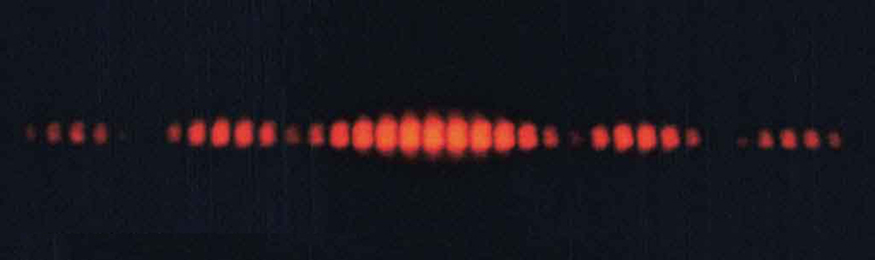
\includegraphics[width=.7\linewidth]{Imagenes/diffraction}
	\caption{Patrón de difracción similar al que debió observar Thomas Young en su experimento de 1801. Imagen recuperada de \parencite{openstax}.}
	\label{fig: double_slit}
\end{figure}